\newcommand{\rightmarkfoot}{\begin{picture}(1,0)\put(0,0.02){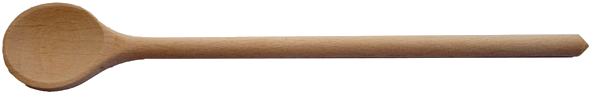
\includegraphics[width=\textwidth,height=1cm]{loeffel1}}\end{picture}}%E
\newcommand{\leftmarkfoot}{\begin{picture}(1,0)\put(0,0.05){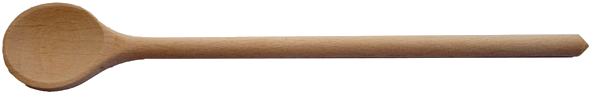
\includegraphics[width=\textwidth,height=1cm,angle=180]{loeffel1}}\end{picture}}%O
\usepackage[a4paper, margin=1in]{geometry}
\usepackage{authblk}
\setcounter{tocdepth}{2}
\usepackage{fancyhdr}
\pagestyle{fancy}
\renewcommand{\chaptermark}[1]{\markboth{#1}{}}
\renewcommand{\sectionmark}[1]{\markright{#1}{}}
\addtolength{\headheight}{2\baselineskip}
\fancyhf{}
%\fancyhead[EL]{\thepage}
\fancyhead[EC]{\thepage}
\fancyhead[ER]{\bfseries\rightmark}
\fancyhead[OL]{\bfseries\leftmark}
\fancyhead[OC]{\thepage}
%\fancyhead[OR]{\thepage}
\fancyfoot[ER]{\bfseries\rightmarkfoot}
\fancyfoot[OL]{\bfseries\leftmarkfoot}
\renewcommand{\headrulewidth}{.5pt}
\renewcommand{\footrulewidth}{.5pt}
\renewcommand{\headrulewidth}{0pt}
\renewcommand{\footrulewidth}{0pt}
\setlength{\unitlength}{\textheight} 
\addtolength{\unitlength}{\footskip} 
\addtolength{\unitlength}{\headsep} 
\addtolength{\unitlength}{2pt} 
%\renewcommand{\headrule}{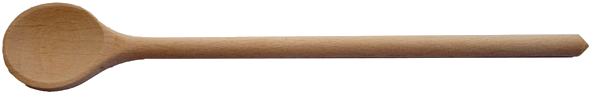
\includegraphics[width=\textwidth,height=2cm]{loeffel1}}
%\renewcommand{\footrule}{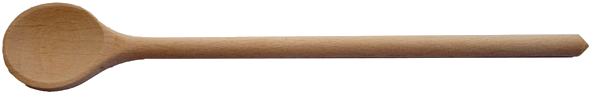
\includegraphics[width=\textwidth,height=2cm,angle=180]{loeffel1}}
\renewcommand{\leftmark}{\begin{picture}(1,0)\put(0,0.008){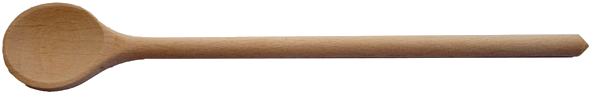
\includegraphics[width=\textwidth,height=1cm,angle=180]{loeffel1}}\end{picture}}%O
\renewcommand{\rightmark}{\begin{picture}(1,0)\put(0,-0.03){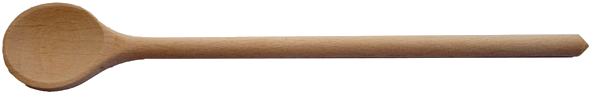
\includegraphics[width=\textwidth,height=1cm]{loeffel1}}\end{picture}}%E
%\renewcommand{\leftmark}{\begin{picture}(1,0)\put(-0.1,0.05){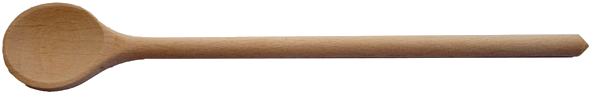
\includegraphics[width=1.2\textwidth,height=2cm,angle=180]{loeffel1}}\end{picture}}%O
%\renewcommand{\rightmark}{\begin{picture}(1,0)\put(-0.02,-0.025){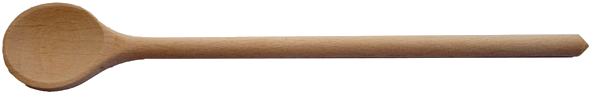
\includegraphics[width=1.2\textwidth,height=2cm]{loeffel1}}\end{picture}}%E
%on chapter and maketitle calls
\fancypagestyle{plain}{%
\fancyhead{}
\renewcommand{\headrulewidth}{0pt}
\renewcommand{\footrulewidth}{0pt}
\fancyfoot[OC]{\thepage}
\fancyfoot[EC]{\thepage}
}
\setlength{\topskip}{0mm}

\makeatletter
\def\thickhrulefill{\leavevmode \leaders \hrule height 1ex \hfill \kern \z@}
\def\@makechapterhead#1{%
  \vspace*{10\p@}%
  {\parindent \z@ \raggedleft \reset@font
            \scshape \@chapapp{} \thechapter
        \par\nobreak
        \interlinepenalty\@M
    \Huge \bfseries #1\par\nobreak
    %\vspace*{1\p@}%
    \hrulefill
    \par\nobreak
    \vskip 100\p@
  }}
\def\@makeschapterfoot#1{%
  \vspace*{10\p@}%
  {\parindent \z@ \raggedleft \reset@font
            \scshape \vphantom{\@chapapp{} \thechapter}
        \par\nobreak
        \interlinepenalty\@M
    \Huge \bfseries #1\par\nobreak
    %\vspace*{1\p@}%
    %\hrulefill
    \par\nobreak
    \vskip 100\p@
  }}
\makeatother

